\section{Dynamic Diagrams}
\label{sec:dynamics}
\subsection{Battle}
\begin{figure}[h]
\center
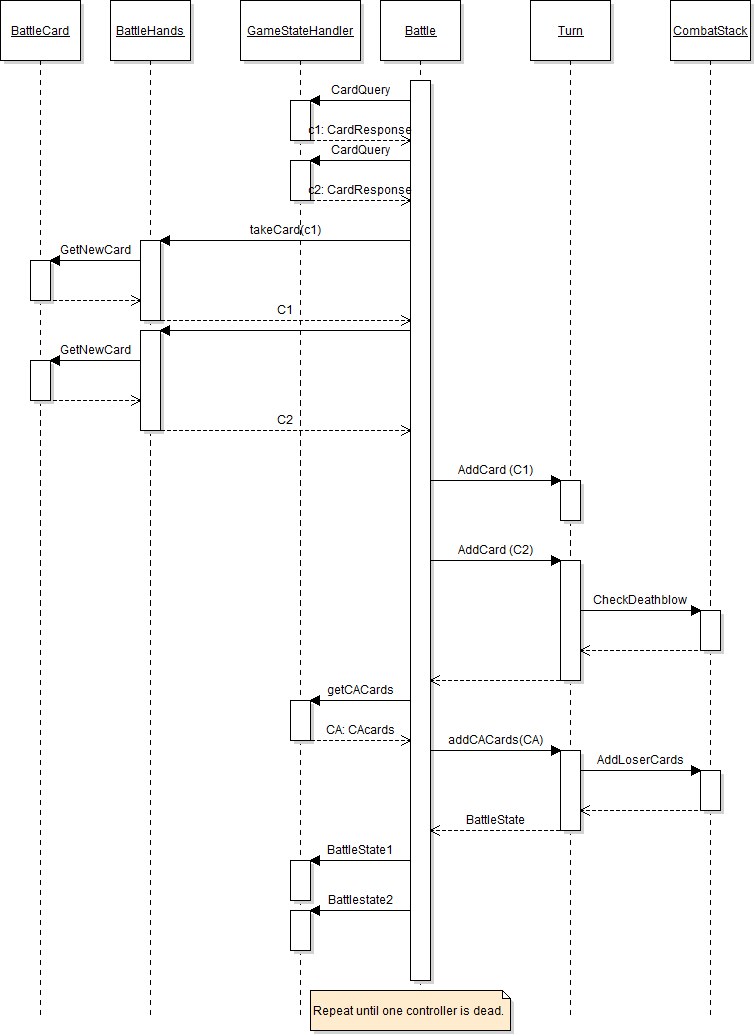
\includegraphics[width=0.9\textwidth]{diagrams/BattleSequenceDiagram.png}
\caption{A sequence diagram of one turn for each participant in a battle.}
\label{fig:battle_sequence_diagram}
\end{figure}

\begin{figure}[h]
\center
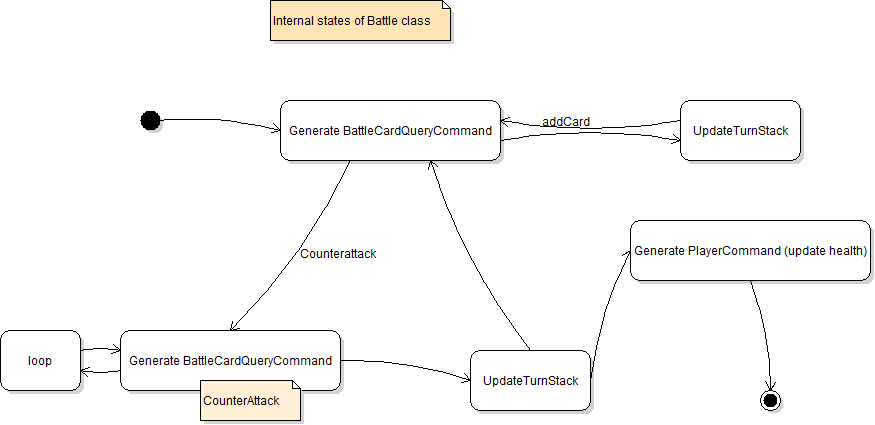
\includegraphics[width=0.9\textwidth]{diagrams/BattleStateDiagram.png}
\caption{A state diagram explaining the internal states of the Battle class.}
\label{fig:battle_state_diagram}
\end{figure}


A battle is conducted between two players controlled either by a human player or by the AI. For more information on how a battle is conducted according to the rules, see use case \ref{fightopponent}.

Figure \ref{fig:battle_sequence_diagram} models one turn in a battle (likely, a full battle would have several turns). The \texttt{GameStateHandler} communicates with human players and the AI through means not shown in this diagram, and the response is in the form of a card in the respective participant's battle hand. The class \texttt{Battle} acts as a mediator between the heroes, their battle hands and \texttt{Turn}. A battle hand is composed of the five cards currently available to the respective player. The \texttt{Turn} class contains the logic determining the winner of a single battle turn by comparing the chosen cards and possible lingering effects from previous rounds (specifically \emph{death blows}, see use case \ref{fight_deathblow}). When a turn ends, the losers' cards are added to the combat stack.

Figure \ref{fig:battle_state_diagram} models the states in which the \texttt{Battle} class will be, from the start until the end of a battle, out of the class's own perspectiv.

\begin{figure}[h]
\center
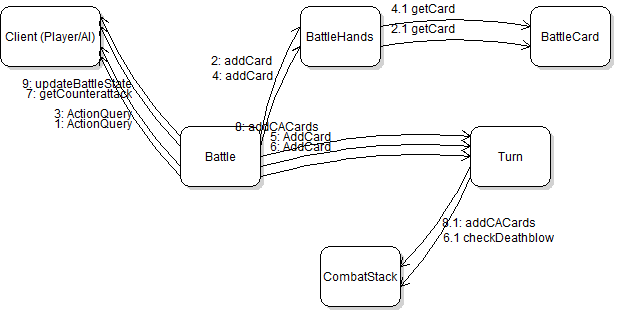
\includegraphics[width=0.9\textwidth]{diagrams/CounterAttackCommDiagram.png}
\caption{A communication diagram explaining the communication between the participating classes.}
\label{fig:counter_attack_comm_diagram}
\end{figure}

A counter attack is possible in each turn for the losing participant given certain circumstances. For more detail on counter attack see use case \ref{fight_counterattack}. Figure \ref{fig:counter_attack_comm_diagram} models the communication between the classes participating in a single turn when a counter attack is possible.


\begin{figure}[h]
\center
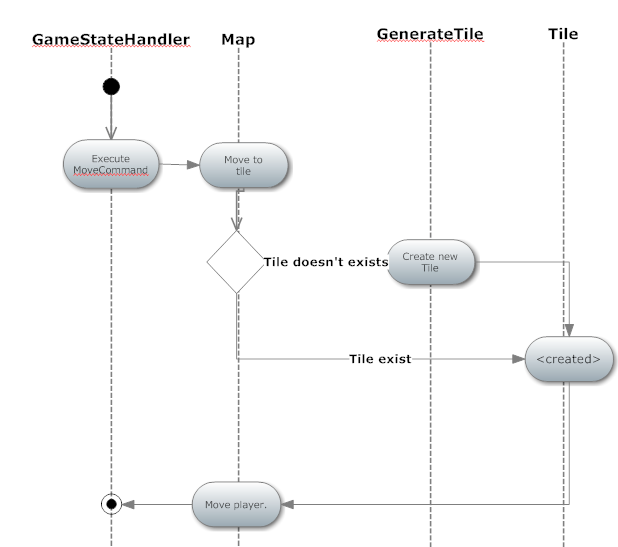
\includegraphics[width=0.9\textwidth]{diagrams/moveActivityDiagram.png}
\caption{An activity diagram explaining the process of a hero moving to a new square and the possible creation of a new tile.}
\label{fig:move_activity_diagram}
\end{figure}

Figure \ref{fig:move_activity_diagram} models the process of a hero moving to a new room. For further information on how a move is carried out, see use case \ref{moveoutfromroom}. A \emph{tile} is created if the room has previously not been visited, otherwise the hero simply moves to the new room.

\begin{figure}[h]
\center
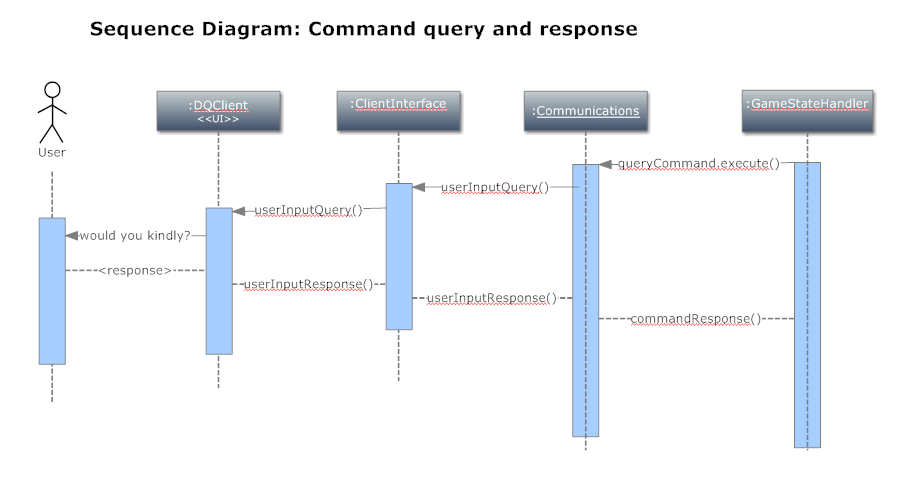
\includegraphics[width=0.9\textwidth]{diagrams/moveCommandSequenceDiagram.png}
\caption{An sequence diagram depicting the how communication is done with the end user.}
\label{fig:randsequence}
\end{figure}

Figure \ref{fig:randsequence} shows how the system asks for input from the user, and receives a reply. The diagram models this from the point when the command gets exectued in the \texttt{GameStateHandler}. Thus it cannot be seen which subsystem requires the user input, which illustrates the fact that the communication behaviour is independent on the other system subsystems.
